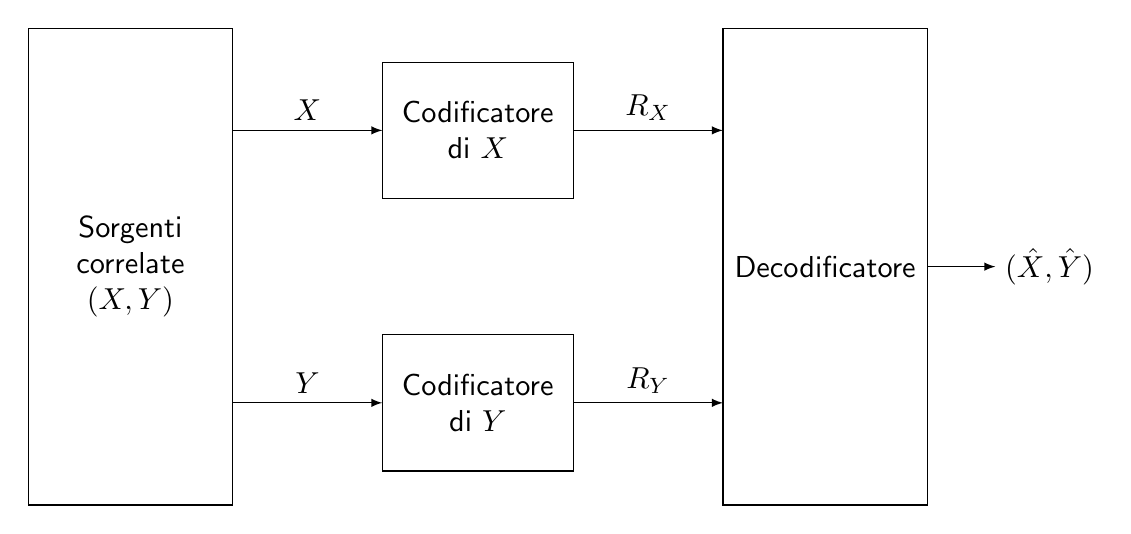
\begin{tikzpicture}[scale=0.865,>=latex]
    \tikzstyle{every node}=[font=\fontsize{11}{13}\sffamily]

    \draw (0,0) rectangle (3,7)
    node[midway,align=center]{Sorgenti \\ correlate \\ \((X,Y)\)};

    \draw[->] (3,5.5) -- (5.2,5.5)
    node[above,midway]{\(X\)};

    \draw[->] (3,1.5) -- (5.2,1.5)
    node[above,midway]{\(Y\)};

    \draw (5.2,4.5) rectangle (8,6.5)
    node[midway,align=center]{Codificatore \\ di \(X\)};

    \draw (5.2,0.5) rectangle (8,2.5)
    node[midway,align=center]{Codificatore \\ di \(Y\)};

    \draw[->] (8,5.5) -- (10.2,5.5)
    node[above,midway]{\(R_X\)};

    \draw[->] (8,1.5) -- (10.2,1.5)
    node[above,midway]{\(R_Y\)};

    \draw (10.2,0) rectangle (13.2,7)
    node[midway]{Decodificatore};

    \draw[->] (13.2,3.5) -- (14.2,3.5)
    node[right]{\((\hat{X},\hat{Y})\)};
\end{tikzpicture}
